\chapter{Bitcoin Lightning network}

Bitcoin is currently far from supporting the world finantial exchanges, it handles about 250.000 transactions in a day, while VISA handles about 47.000 transactions \textit{per second}.
This is due mainly to max block size and block time, that are respectively 1MB and 10 minutes, and also to the need of broadcasting a transaction to every node.
\texttt{
BitcoinCash} forked from Bitcoin to increase the block size to 8MB, and then to 32MB, but this is not a definitive solution, because the block size can't be increased indefinitely, and the network would be more centralized, since each year every node would have to store about 400TB of data.

\section{Introduction}
The idea behind the \textbf{Lightning Network} is to create a second layer on top of the Bitcoin blockchain, where transactions are not broadcasted to the network, but are settled on the main chain only when necessary.

A customer may deposit money on a separate \textit{payment channel}, where payments are registered in private ledgers handled by the ``merchant''.
Every time that the customer buys something, he sends a new transaction replacing the precedent one.
The merchant doesn't risk anything because he can commit the transaction on the blockchain at any time, and the customer can't spend more than he has deposited.

In general opening a new channel is a transaction, so it is not optimal to create a new channel every time a customer has to send a payment; this is why the Lightning Network uses a \textbf{network of channels}, where a customer can send a payment to a merchant through a series of ---existing--- channels.
\note{
If one of the two parties cheats all the channel funds are granted to
counterparty.}

\subsection{How it works}
\begin{enumerate}


   \item \textit{Opening a Lightning Channel}:
   Let’s say Alice wants to pay Bob with Bitcoin. To establish a payment channel, Alice or Bob (or both) must deposit Bitcoin into a 2-of-2 multi-signature (multisig) wallet2. This is like opening a tab at a bar. You pay some money upfront, and then you can make many transactions (buying drinks) without having to reach for your wallet each time.

   \item \textit{Transacting in the Lightning Channel}:
   Now that there is funding available, Alice can send the payment to Bob2. These transactions happen off-chain, meaning they don’t need to be recorded on the Bitcoin blockchain. This allows for faster and cheaper transactions.
   Both of them have a signed copy of the latest state of the channel.

   \item \textit{Closing the Lightning Channel}:
   When Alice and Bob are done transacting, they can close the channel. This involves settling the final state of their transactions on the Bitcoin blockchain. This is like closing your tab at the bar. You settle the final bill based on all the drinks you’ve had.

\end{enumerate}

\section{Punishing cheaters}
The first issue is that m\ul{id-transactions are valid even in case there are newer ones}.
There is no way for thr Lightning network to guarantee to rip up older transactions when a new one is created.
The current workaround is based on \textbf{punishment}:
\begin{itemize}
   \item Transactions have a ``revocation secret'', which is sent to Bob by Alice when she creates a new transaction.
   \item In case Alice publishes a newer transaction, Bob can use the revocation secret to redeem all the funds in the channel.
\end{itemize}
The protocol must give time to Bob to check that Alice is cheating to punish her, so there is usually a 24h delay added to these transactions.

\section{Multi-hop payments}
\subsection{HTLC}
HTLC stands for \textit{Hashed TimeLock Contract}, and is a contract that enforces a transaction to be completed within a certain time frame, or the funds are refunded.

This is used in case multiple channels are involved in a transaction, to ensure that the transaction is completed.

\begin{figure}[htbp]
   \centering
   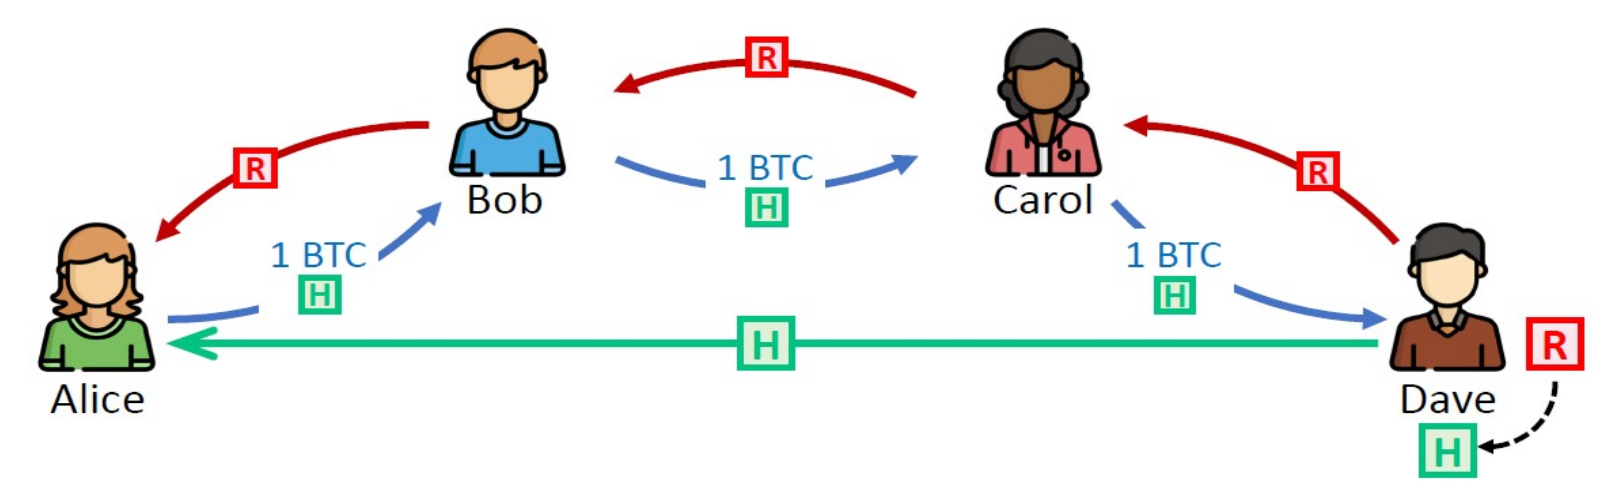
\includegraphics{images/lightning_HTLC1.png}
   \caption{Multi hop payments}
   \label{fig:lightning_HTLC1}
\end{figure}

In this scenario, Alice wants to pay Dave, but they don't have a direct channel.
\begin{enumerate}
   \item Dave generates a secret R and sends H = hash(R) to Alice.
   \item Alice sends a \textit{hash-locked} payment to Bob, with the condition that Bob can redeem the funds only if he knows R.
   \item Each node generates a \textit{hash-locked} payment to the next node, with the same condition.
   \item Dave redeems the payment by revealing R to Carol, who reveals R to Bob, who reveals R to Alice.
   \item When Alice knows R, she knows that every node in the path has been paid.
\end{enumerate}

The \textit{time-locked} part of the contract is used to ensure that Dave propagates R when he receives its Bitcoin within a certain time frame, if he doesn't the funds are refunded to the transferor.

\subsection{Routing}
The problem of paying someone shifts to finding a route between two nodes.\\
LN uses a \textbf{source routing} algorithm, where the source node knows the whole network and can find the shortest path to the destination, it is a BGP-like solution.
To ensure privacy, Alice can use \textbf{Onion Routing}, where the payment is encrypted multiple times, and each node in the path can only decrypt the outer layer.

Channels also have fixed capacity, so the network must be balanced to allow for payments in both directions. 
If payment fails because of a lack of capacity, the payment is refunded to Alice, and she tries another route.

\section{Doubts}
It has not been proved yet that the Lightning Network is \textbf{Scalable}, \textbf{Decentralized} and \textbf{Secure} at an acceptable level.

Many problems are still open:
\begin{itemize}
   \item You cannot just ``enter the network'', you need a payment channel, which is costful.
   \item Longer the route, longer the chances of delay
   \item Need for routing algorithms
   \item If there isn't a watchtower, nodes must be online all the time to protect against fraudolent channel closing; on the other hand the watchtower must be trusted.
   \item Counterparty misbehaviour can leave coins locked for a long time
\end{itemize}